% =============================================================================
% cs-fsm-automaton.tex — Finite automaton (DFA) with start and accepting states
%
% Shows: a 3-state DFA over {0,1} accepting exactly those strings that END in
% "01". State meaning: q0 = last symbol was 1 (or nothing yet), q1 = last
% symbol was 0, q2 = last two symbols were 01 (accepting).
% Compiles standalone via: xelatex cs-fsm-automaton.tex
%
% Use for: theory of computation, compilers (lexer DFAs), digital logic (state
% machines), sequential-circuit design.
% =============================================================================

\documentclass[border=4pt]{standalone}
\usepackage{tikz}
\usetikzlibrary{arrows.meta, positioning, automata}

\definecolor{node-fill}{HTML}{E8EDF5}
\definecolor{node-border}{HTML}{012169}
\definecolor{arrow}{HTML}{1A1A1A}
\definecolor{accept}{HTML}{15803D}

\tikzset{
  fsm-state/.style={
    circle, draw=node-border, fill=node-fill, thick,
    minimum size=1.0cm, align=center, font=\small
  },
  fsm-accept/.style={
    circle, draw=accept, fill=node-fill, thick, double, double distance=1.2pt,
    minimum size=1.0cm, align=center, font=\small
  },
  fsm-edge/.style={-{Latex[length=2.5mm]}, thick, draw=arrow, font=\small}
}

% -----------------------------------------------------------------------------
% Diagram: DFA accepting strings ending in "01".
% Coordinates: (x, y)
%   q0 at (0, 0)  -- start state, last symbol was 1 / nothing
%   q1 at (3, 0)  -- last symbol was 0
%   q2 at (6, 0)  -- accepting: last two symbols were 01
% All states are 1.0cm circles (P1: explicit minimum size).
% Forward edges run straight along y=0 with labels ABOVE the line.
% Self-loops sit ABOVE their node (clear of the edge labels, different x).
% The two BACK edges are routed BELOW with explicit out/in angles rather than
% `bend`, so their depth is predictable and they cannot collide with q1:
%   q2->q1 shallow arc (out=210,in=330); q2->q0 deeper arc (out=250,in=290).
% Every edge label carries a directional keyword (P4).
% -----------------------------------------------------------------------------

\begin{document}
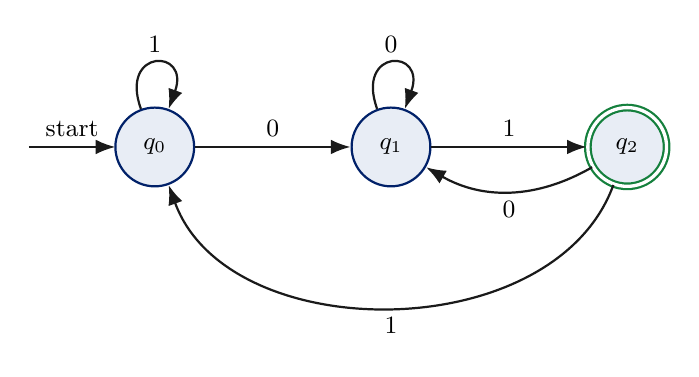
\begin{tikzpicture}
  % Start arrow into q0
  \draw[fsm-edge] (-1.6, 0) -- node[above] {start} (-0.5, 0);

  \node[fsm-state]  (q0) at (0, 0) {$q_0$};
  \node[fsm-state]  (q1) at (3, 0) {$q_1$};
  \node[fsm-accept] (q2) at (6, 0) {$q_2$};

  % Forward transitions
  \draw[fsm-edge] (q0) -- node[above] {0} (q1);
  \draw[fsm-edge] (q1) -- node[above] {1} (q2);

  % Self-loops (above each node)
  \draw[fsm-edge] (q0) to[out=110, in=70, looseness=6] node[above] {1} (q0);
  \draw[fsm-edge] (q1) to[out=110, in=70, looseness=6] node[above] {0} (q1);

  % Back transitions, routed below with explicit angles
  \draw[fsm-edge] (q2) to[out=210, in=330] node[below] {0} (q1);
  \draw[fsm-edge] (q2) to[out=250, in=290] node[below] {1} (q0);
\end{tikzpicture}
\end{document}
